\documentclass[main.tex]{subfiles}

\begin{document}
\chapter{Phonon mediated tunneling into \TaS (BETTER TITLE NEEDED)}\label{ch:sts_gap_tas2}

\section{Amplitude mode in \TaS}

\begin{figure}[h!]
    \centering
    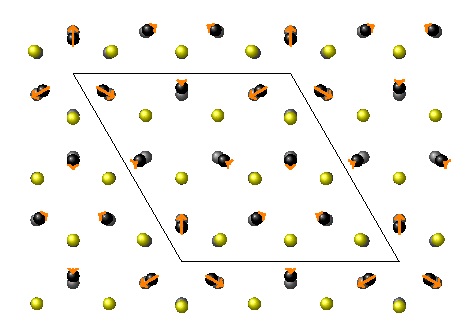
\includegraphics[width=0.75\textwidth]{higgs.pdf}
    \label{}
    \caption{}
\end{figure}

% analyse the mode a bit

\section{Scanning Tunneling Spectroscopy}

\acrfull{sts} is an experimental technique in which a \acrfull{stm} is used to map the density of states of a material.

\todo{introduction stm/sts}

Stipe et al. noted that the tunneling current in \acrshort{sts} can also identify phonon modes of the material measured \cite{stipe_single-molecule_1998} (vibrational modes of a single molecule in this case).

\section{Phonon mediated tunneling in Graphene}

A gap feature around the fermi level in the measured DOS on graphene \cite{zhang_giant_2008} was explained with electron-phonon interaction \cite{wehling_phonon-mediated_2008}.

The underlying mechanism is that electrons can elastically tunnel into graphene at the Fermi level near the \(\vb{K}\) point. \todo{Graphic for that would be nice}
This elastic process is suppressed because the wave function at the initial state i.e. the wave functions at the tip have a momentum distribution centered at \(\vb*{k}_{\parallel} = 0\), so the tunneling matrix element is suppressed for large \(\vb*{k}\) \cite{vitali_phonon_2004}.
For electron energies larger than the energy 

\section{Phonon mediated tunneling into \TaS}

In a 2019 paper by Hall et al. \cite{hall_environmental_2019}, a similar gap feature with a width of \(2 \Delta = \SI[separate-uncertainty = true]{32 \pm 9}{\milli\eV}\) was recorded in an \acrshort{sts} measurement on \TaS.

This gap is attributed to partial gapping to the formation of the charge density wave.
\todo{explain cdw phase, gap due to peierls somewhere, reference here}

\begin{figure}[htb!]
    \centering
    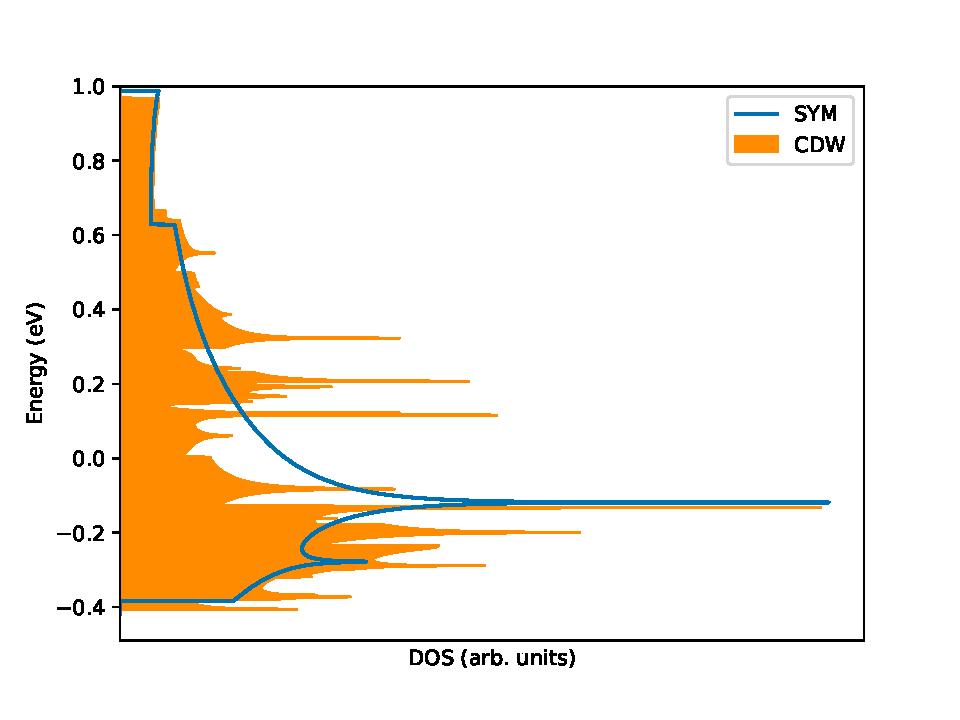
\includegraphics[width=0.6\textwidth]{tas2_dos.pdf}
    \caption{Density of states for \TaS in the charge density wave (CDW) and undistorted (SYM) phase. The data was kindly provided by Dr.\,Jan Berges and has been calculated using the 2D tetrahedron method using 360² (1080²) k points for the CDW (SYM) structure}
    \label{fig:tas2_dos}
\end{figure}
\todo{woher kommt die genau? Quantum Espresso?}
The density of states shown in fig. \ref{fig:} shows no symmetric gap around the Fermi level.


\end{document}